\documentclass[aspectratio=149]{beamer}

\usepackage[utf8]{inputenc}
\usepackage{setspace}
\usepackage{amsmath}
\usepackage{amsthm}
\usepackage{amssymb}
\usepackage{xcolor}

\title{T.C.A.S.}
\author[Roberto Bertolini]{Roberto Alessandro Bertolini}
\institute[Liceo Nervi Ferrari]{Liceo "P. Nervi - G. Ferrari" - Morbegno}
\date{Giugno 2021}
\subtitle{TCAS Can Always Solve}

\usetheme{Berlin}
\setbeamertemplate{mini frames}{} 
\usecolortheme{default}
%&\usefonttheme{serif}


\makeatletter
\setbeamertemplate{headline}{%
	\begin{beamercolorbox}[colsep=1.5pt]{upper separation line head}
	\end{beamercolorbox}
	\begin{beamercolorbox}{section in head/foot}
		\vskip2pt\insertsectionnavigationhorizontal{\paperwidth}{}{}\vskip2pt
	\end{beamercolorbox}%
	\ifbeamer@theme@subsection%
	%\begin{beamercolorbox}[colsep=1.5pt]{middle separation line head}
	%\end{beamercolorbox}
	%\begin{beamercolorbox}[ht=2.5ex,dp=1.125ex,%
	%	leftskip=.3cm,rightskip=.3cm plus1fil]{subsection in head/foot}
	%	\usebeamerfont{subsection in head/foot}\insertsubsectionhead
	%\end{beamercolorbox}%
	\fi%
	\begin{beamercolorbox}[colsep=1.5pt]{lower separation line head}
	\end{beamercolorbox}
}
\makeatother

\setbeamertemplate{caption}{\raggedright\insertcaption\par}

\begin{document}
	
	\begin{frame}
		\titlepage
	\end{frame}
	
	%\begin{frame}
	%	\frametitle{Indice}
	%	\tableofcontents
	%\end{frame}
	
	\section{Introduzione}
	
	\subsection{La definizione di limite}
	\begin{frame}
		\frametitle{La definizione di limite}
		\begin{block}{Definizione generale di limite di una funzione}
			\[ 
			\lim_{x \to x_{0}}{f(x) = l} 
			\]
			
			Se \( 
			\forall \varepsilon > 0 \enspace \exists \enspace \delta(\varepsilon) \mid \forall x \in D_{f}, 0 < \: \mid x - x_{0} \mid \: <\delta \implies \mid f(x) - l \mid < \varepsilon
			\)
		\end{block}
		\onslide<2>\begin{exampleblock}{Esempio}
			\[
				\lim_{x \to 3}{x^2} = 9; \quad \lim_{x \to +\infty}{\frac{1}{x}} = 0
			\]
		\end{exampleblock}
	\end{frame}
	
	\subsection{La risoluzione per approssimazione}
	\begin{frame}
		\frametitle{La risoluzione per approssimazione}
		\begin{columns}
			\begin{column}{0.5\textwidth}
				Consideriamo \(
					f(x) = \frac{1}{x^{\ln{\ln{\ln{\ln{\frac{1}{x}}}}}-1}}
				\)\\
				
				\vspace{5mm}
				\onslide<2-7>{Cerchiamo \(\lim_{x \to 0^{+}}{f(x)}\)}
				\onslide<8->{\\Cerchiamo \(\lim_{x \to 0^{+}}{f(x)} = 0\)}
				
				\vspace{5mm}
				\onslide<8->{
					Eppure \(\lim_{x \to 0^{+}}{f(x)} = +\infty\)
				}
			
				\vspace{5mm}
				\onslide<9>{
					La funzione ha un minimo in \(x \approx 4.29 \times 10 ^{-1656521}\)
				}
			
			\end{column}
			\begin{column}{0.5\textwidth}
				\begin{figure}
					\begin{overprint}
						\onslide<2>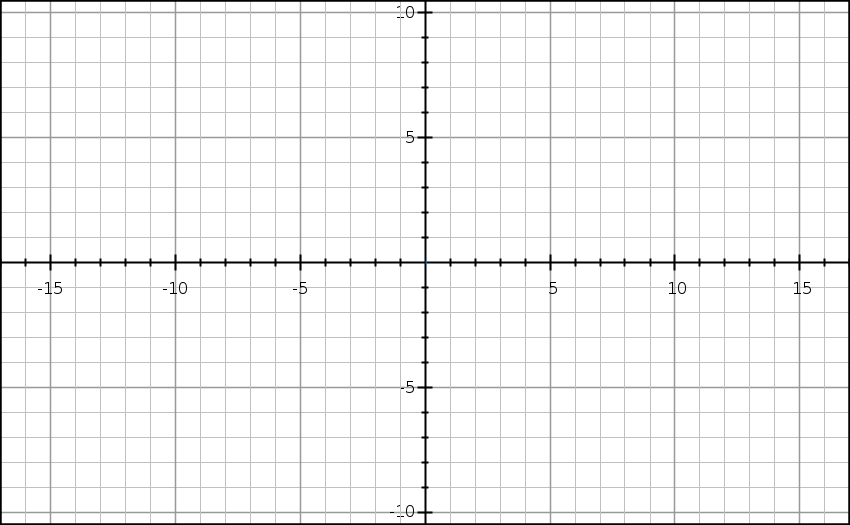
\includegraphics[width=\textwidth]{pres_img/f1.png}
						\onslide<3>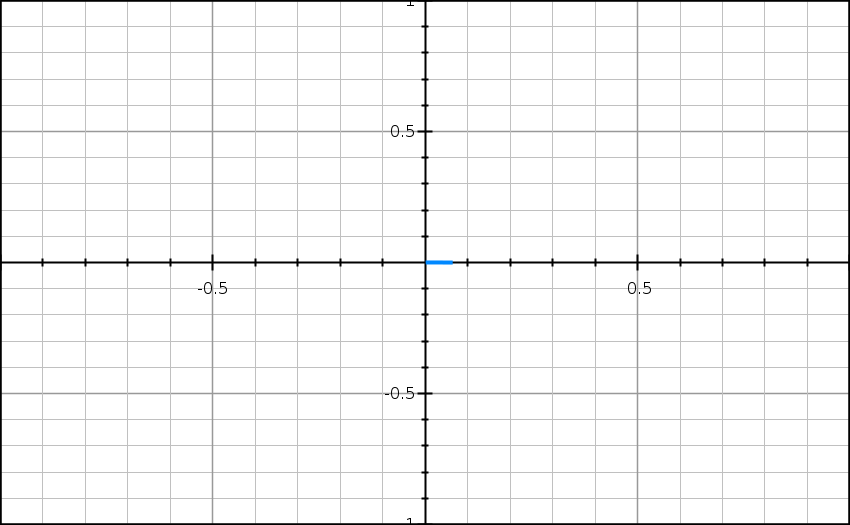
\includegraphics[width=\textwidth]{pres_img/f2.png}
						\onslide<4>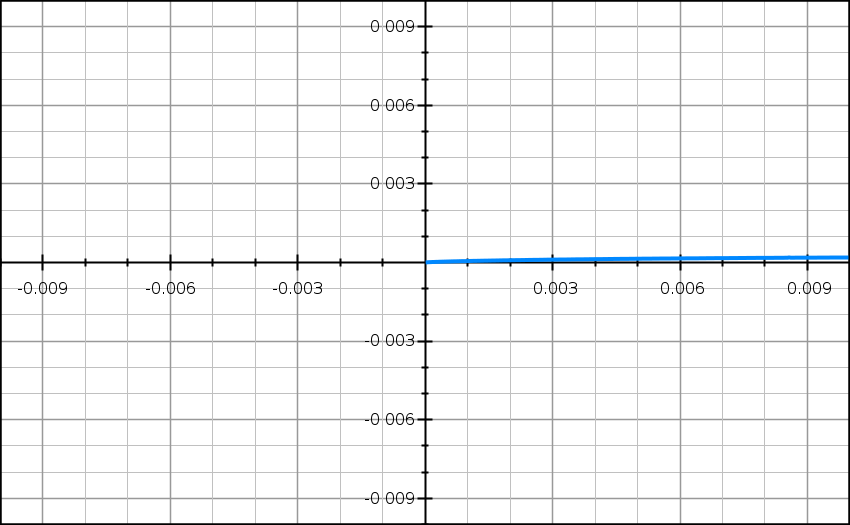
\includegraphics[width=\textwidth]{pres_img/f3.png}
						\onslide<5>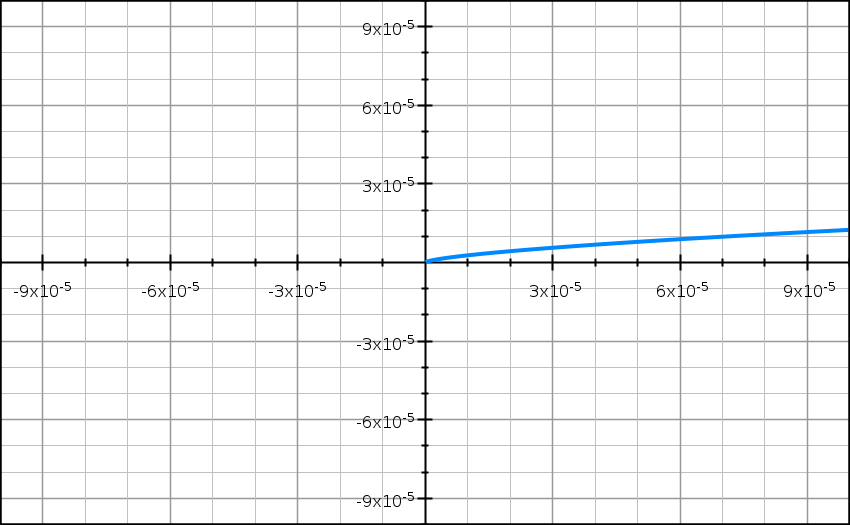
\includegraphics[width=\textwidth]{pres_img/f4.png}
						\onslide<6>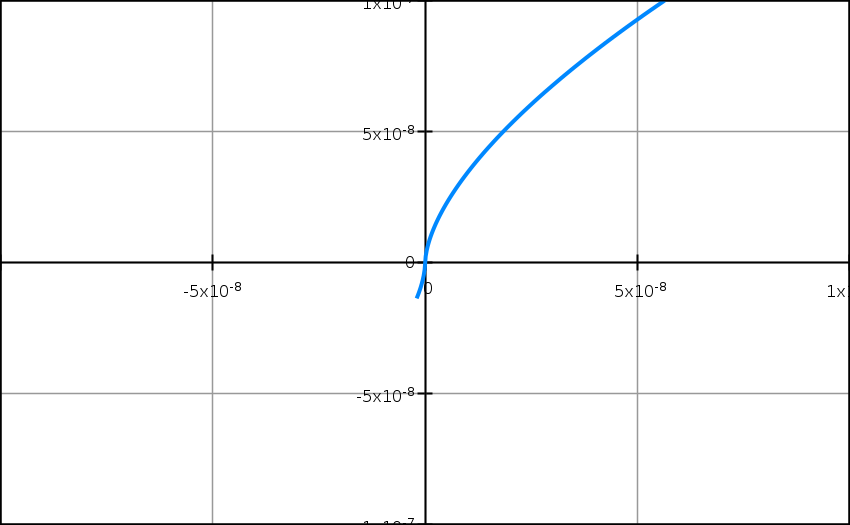
\includegraphics[width=\textwidth]{pres_img/f5.png}
						\onslide<7->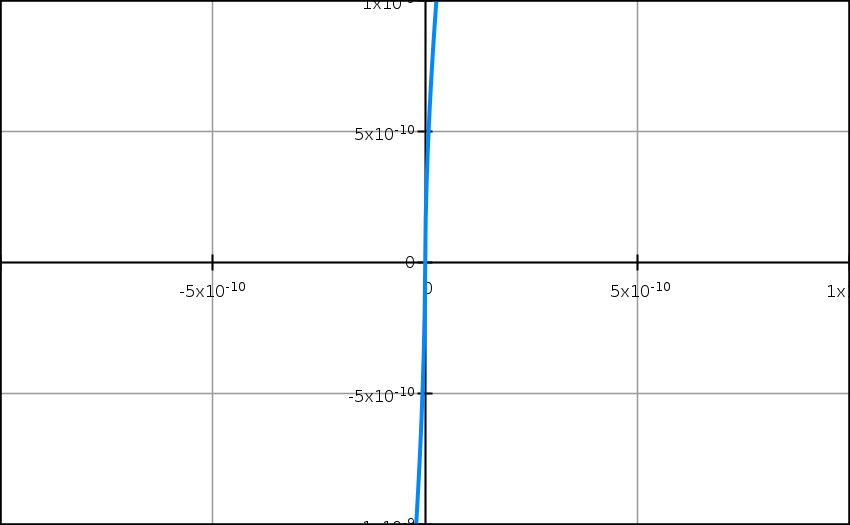
\includegraphics[width=\textwidth]{pres_img/f6.png}
					\end{overprint}
				\end{figure}
			\end{column}
		\end{columns}
	\end{frame}
	
	\subsection{L'approccio matematico}
	\begin{frame}
		\frametitle{L'approccio matematico}
		\begin{block}{La regola di De L'Hôpital}
			\[
			\begin{aligned}
				\text{Se} &\lim_{x \to x_{0}}{f(x)} = \lim_{x \to x_{0}}{g(x)} = 0 \\ \text{oppure} &\lim_{x \to x_{0}}{\lvert f(x) \rvert} = \lim_{x \to x_{0}}{\lvert g(x) \rvert} = \infty \\ \text{ed esiste} &\lim_{x \to x_{0}}{\frac{f'(x)}{g'(x)}} = l \in \mathbf{R} \\ \text{allora} &\lim_{x \to x_{0}}{\frac{f(x)}{g(x)}} = l
			\end{aligned}
			\]
		\end{block}
	\end{frame}

	\begin{frame}
		\frametitle{I problemi dell'approccio matematico}
		\begin{block}{La regola di De L'Hôpital}
			\[
			\lim_{x \to x_{0}}{\frac{f(x)}{g(x)}} = \lim_{x \to x_{0}}{\frac{f'(x)}{g'(x)}}
			\]
		\end{block}
		\onslide<2>\begin{alertblock}{Esempio}
			\[
			f(x) = e^{x} + e^{-x}
			\] 
			\[
			g(x) = e^{x} - e^{-x}
			\]	
			\[
			\lim_{x \to \infty}{\frac{f''(x)}{g''(x)}} = \lim_{x \to \infty}{\frac{e^{x} + e^{-x}}{e^{x} - e^{-x}}} = \lim_{x \to \infty}{\frac{f(x)}{g(x)}}; \quad \lim_{x \to \infty}{\frac{f'(x)}{g'(x)}} = \lim_{x \to \infty}{\frac{e^{x} - e^{-x}}{e^{x} + e^{-x}}}
			\]
		\end{alertblock}
	\end{frame}

	\subsection{La notazione polacca}
	\begin{frame}
		\frametitle{La notazione polacca}
		\begin{block}{Notazione Polacca}
			È una notazione prefissa in cui gli operatori sono a sinistra degli argomenti. Non richiede parentesi perché non presenta ambiguità nell'interpretazione, se degli operatori è nota l'arietà.
		\end{block}
		\onslide<2->\begin{exampleblock}{Esempio}
			\onslide<2->{\[
				3 \times (4 - 5) \rightarrow \times \: 3 - 4 \: 5
			\]}
			\onslide<3->{\[
				\lim_{\textcolor{red}{x} \to \textcolor{blue}{0}}{\frac{\textcolor{orange}{e^{x} - 1}}{x}} \rightarrow \text{lim} \: / \textcolor{orange}{- \text{exp} \: x \: 1} \: x \: \textcolor{red}{x} \: \textcolor{blue}{0}
			\]}
		\end{exampleblock}
	\end{frame}
	
	\section{TCAS}
	
	\subsection{Il parsing dell'espressione}
	\begin{frame}
		\frametitle{Il parsing dell'espressione}
		\only<1>{\[
			\lim_{x \to 0}{\frac{\sin{x}}{x}}
		\]}
		\visible<2-3>{
			\begin{center}
				lim \slash \: sin x x x 0
			\end{center}
		}
		\onslide<3->{
			\begin{center}$\downarrow$\end{center}
			\begin{figure}
				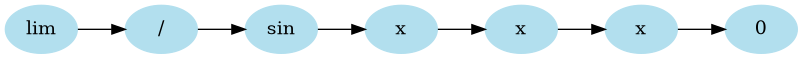
\includegraphics[width=0.8\textwidth]{pres_img/token.png}
			\end{figure}
		}
	\end{frame}
	
	\begin{frame}
		\begin{figure}
			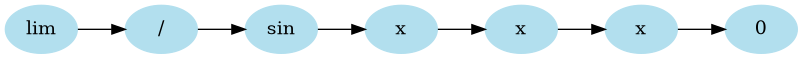
\includegraphics[width=0.8\textwidth]{pres_img/token.png}
		\end{figure}
		\onslide<2>{
			\begin{center}$\downarrow$\end{center}
			\begin{figure}
				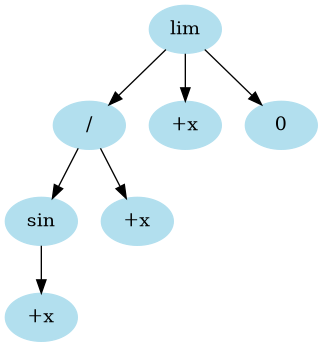
\includegraphics[width=0.3\textwidth]{pres_img/start.png}
				\caption{\(\lim_{x \to 0}{\frac{\sin{x}}{x}}\)}
			\end{figure}
		}
	\end{frame}

	\subsection{Riformulazione del limite}
	
	\begin{frame}
		\begin{columns}
			\begin{column}{0.45\textwidth}
				\begin{figure}
					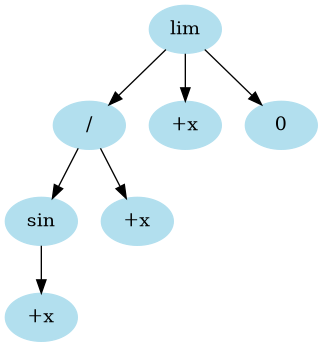
\includegraphics[width=0.8\textwidth]{pres_img/start.png}
					\caption{\(\lim_{x \to 0}{\frac{\sin{x}}{x}}\)}
				\end{figure}
			\end{column}
			\begin{column}{0.1\textwidth}
				\begin{center}
					$\rightarrow$
				\end{center}
			\end{column}
			\onslide<2>\begin{column}{0.45\textwidth}
				\begin{figure}
					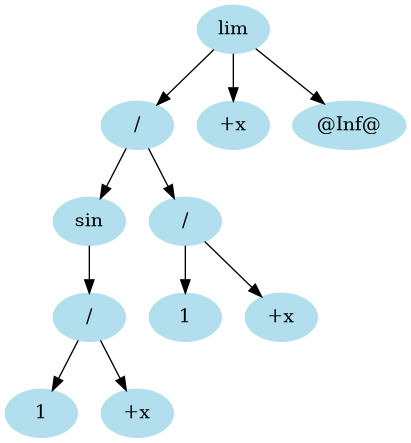
\includegraphics[width=0.8\textwidth]{pres_img/riformulato.png}
					\caption{\(\lim_{x \to +\infty}{\frac{\sin{\frac{1}{x}}}{\frac{1}{x}}}\)}
				\end{figure}
			\end{column}
		\end{columns}
	\end{frame}

	\subsection{Prima semplificazione}
	
	\begin{frame}
		\begin{columns}
			\begin{column}{0.45\textwidth}
				\begin{figure}
					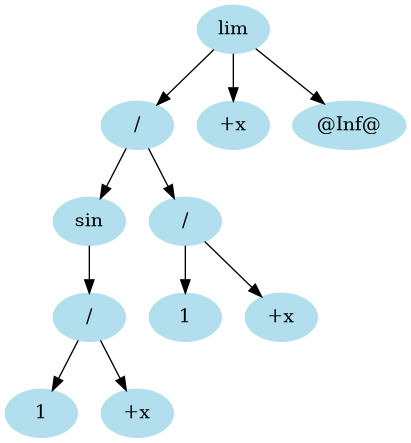
\includegraphics[width=0.8\textwidth]{pres_img/riformulato.png}
					\caption{\(\lim_{x \to +\infty}{\frac{\sin{\frac{1}{x}}}{\frac{1}{x}}}\)}
				\end{figure}
			\end{column}
			\begin{column}{0.1\textwidth}
				\begin{center}
					$\rightarrow$
				\end{center}
			\end{column}
			\onslide<2>\begin{column}{0.45\textwidth}
				\begin{figure}
					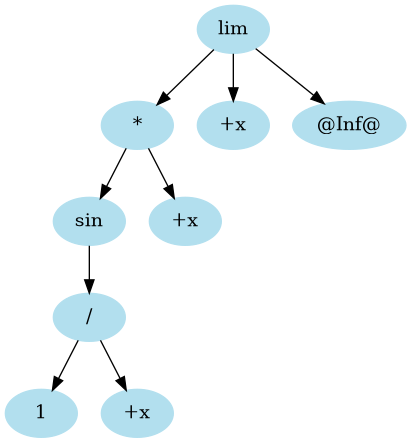
\includegraphics[width=0.8\textwidth]{pres_img/prima_semplif.png}
					\caption{\(\lim_{x \to +\infty}{\sin{\frac{1}{x}} \cdot x}\)}
				\end{figure}
			\end{column}
		\end{columns}
	\end{frame}

	\subsection{Determinazione dell'MRV}
	
	\begin{frame}
		\begin{block}{Sottoespressione di una funzione}
			Una funzione \(g(x)\) è detta sottoespressione di un'altra \(f(x)\) se deve essere valutata per determinare il valore di \(f(x)\)
			\[
			\begin{aligned}
				g(x) \triangleleft f(x)&\text{, se} \: g(x) \: \text{è una sottoespressione di} \: f(x) \\
				g(x) \ntriangleleft f(x)&\text{, se} \: g(x) \: \text{non è una sottoespressione di} \: f(x)
			\end{aligned}
			\]
		\end{block}
		\begin{block}{Classe di Comparabilità}
			\[
			\begin{aligned}
				f(x) \prec g(x) \: \text{se e solo se} \enspace &\lim_{x \to \infty}{\frac{\ln{\mid f(x)\mid}}{\ln{\mid g(x)\mid}}} = 0 \\ 
				f(x) \asymp g(x) \: \text{se e solo se} \enspace &\lim_{x \to \infty}{\frac{\ln{\mid f(x)\mid}}{\ln{\mid g(x)\mid}}} \neq 0 \in \mathbf{R}
			\end{aligned}
			\] 
		\end{block}
	\end{frame}

	\begin{frame}
		\frametitle{Definizione di MRV}
		\begin{block}{MRV}
			È l'insieme di sottoespressioni della funzione con la più alta classe di comparabilità.
			\[
			mrv(f(x)) = \begin{cases}
				\{\} \quad \text{if} \enspace x \ntriangleleft f(x) \\
				\{g(x) \mid g(x) \triangleleft f(x) \wedge (\nexists \enspace h(x) \triangleleft f(x) \mid h(x) \succ g(x)))\}
			\end{cases}
			\]
		\end{block}
	\end{frame}

	\begin{frame}
		\begin{columns}
			\begin{column}{0.45\textwidth}
				\begin{figure}
					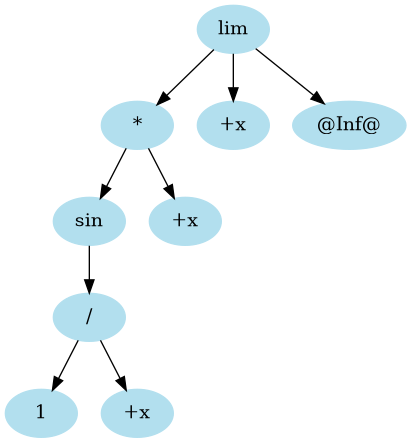
\includegraphics[width=0.8\textwidth]{pres_img/prima_semplif.png}
					\caption{\(\lim_{x \to +\infty}{\sin{\frac{1}{x}} \cdot x}\)}
				\end{figure}
			\end{column}
			\begin{column}{0.1\textwidth}
				\begin{center}
					$\rightarrow$
				\end{center}
			\end{column}
			\onslide<2>\begin{column}{0.45\textwidth}
				\begin{figure}
					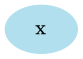
\includegraphics[width=0.2\textwidth]{pres_img/mrv_1.png}
					\caption{\(x\)}
				\end{figure}
			\end{column}
		\end{columns}
	\end{frame}

	\subsection{Riscrittura del limite}
	
	\begin{frame}
		\frametitle{Incrementare la classe di comparabilità}
		\begin{block}{Limite di un limite}
			\[
			\lim_{x \to +\infty}{f(x)}=+\infty \:, \: \lim_{x \to +\infty}{g(x)}=+\infty \implies \lim_{x \to +\infty}{f(g(x))}=+\infty
			\]
		\end{block}
		\begin{exampleblock}{Esempio}
			\[
				\lim_{x \to +\infty}{\sin{\frac{1}{x}} \cdot x} = \lim_{x \to +\infty}{\sin{e^{-x}} \cdot e^{x}}
			\]
		\end{exampleblock}
	\end{frame}

	\begin{frame}
		\begin{columns}
			\begin{column}{0.45\textwidth}
				\begin{figure}
					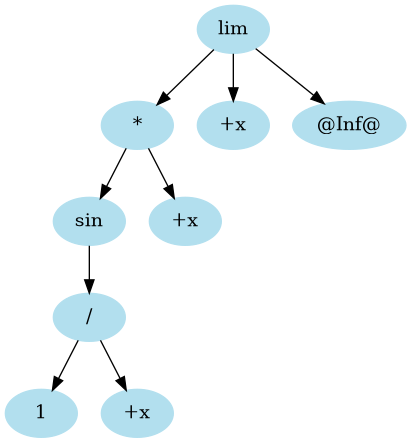
\includegraphics[width=0.8\textwidth]{pres_img/prima_semplif.png}
					\caption{\(\lim_{x \to +\infty}{\sin{\frac{1}{x}} \cdot x}\)}
				\end{figure}
			\end{column}
			\begin{column}{0.1\textwidth}
				\begin{center}
					$\rightarrow$
				\end{center}
			\end{column}
			\onslide<2>\begin{column}{0.45\textwidth}
				\begin{figure}
					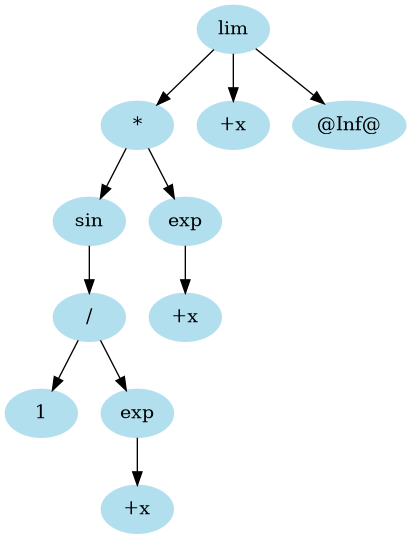
\includegraphics[width=0.8\textwidth]{pres_img/replaced.png}
					\caption{\(\lim_{x \to +\infty}{\sin{\frac{1}{e^{x}}} \cdot e^{x}}\)}
				\end{figure}
			\end{column}
		\end{columns}
	\end{frame}

	\subsection{Seconda semplificazione}
	
	\begin{frame}
		\begin{columns}
			\begin{column}{0.45\textwidth}
				\begin{figure}
					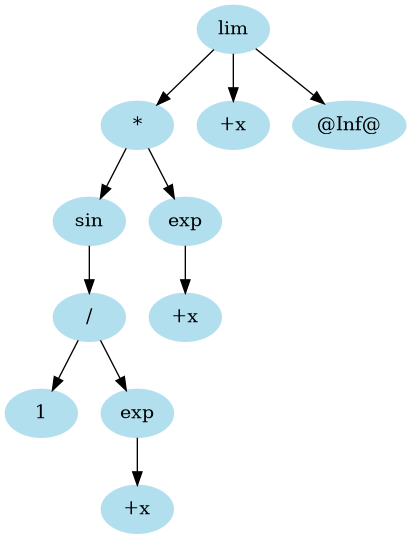
\includegraphics[width=0.8\textwidth]{pres_img/replaced.png}
					\caption{\(\lim_{x \to +\infty}{\sin{\frac{1}{e^{x}}} \cdot e^{x}}\)}
				\end{figure}
			\end{column}
			\begin{column}{0.1\textwidth}
				\begin{center}
					$\rightarrow$
				\end{center}
			\end{column}
			\onslide<2>\begin{column}{0.45\textwidth}
				\begin{figure}
					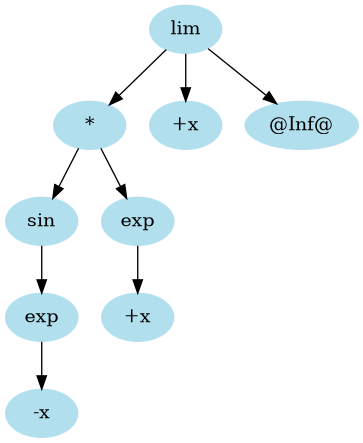
\includegraphics[width=0.8\textwidth]{pres_img/simplified2.png}
					\caption{\(\lim_{x \to +\infty}{\sin{e^{-x}} \cdot e^{x}}\)}
				\end{figure}
			\end{column}
		\end{columns}
	\end{frame}

	\subsection{Determinazione del nuovo MRV}
	
	\begin{frame}
		\begin{columns}
			\begin{column}{0.45\textwidth}
				\begin{figure}
					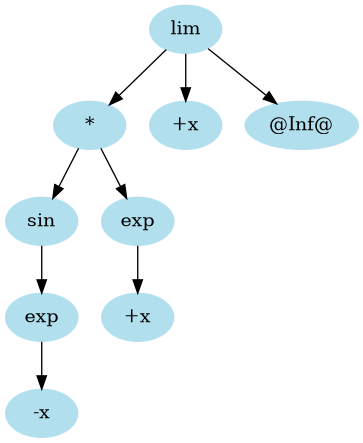
\includegraphics[width=0.8\textwidth]{pres_img/simplified2.png}
					\caption{\(\lim_{x \to +\infty}{\sin{e^{-x}} \cdot e^{x}}\)}
				\end{figure}
			\end{column}
			\begin{column}{0.1\textwidth}
				\begin{center}
					$\rightarrow$
				\end{center}
			\end{column}
			\onslide<2>\begin{column}{0.45\textwidth}
				\begin{figure}
					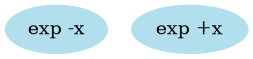
\includegraphics[width=0.5\textwidth]{pres_img/mrv_2.png}
					\caption{\(e^{-x}, e^{x}\)}
				\end{figure}
			\end{column}
		\end{columns}
	\end{frame}
	
	\begin{frame}
		\begin{exampleblock}{Sostituzione}
			Posto \(w = e^{-x}\)
		\end{exampleblock}
		\begin{columns}
			\begin{column}{0.45\textwidth}
				\begin{figure}
					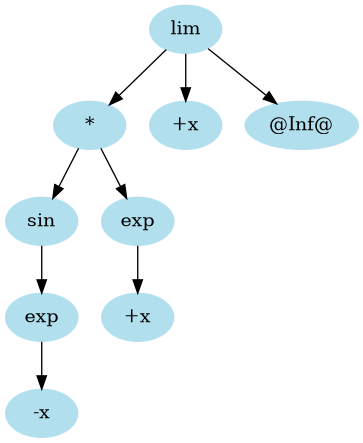
\includegraphics[width=0.8\textwidth]{pres_img/simplified2.png}
					\caption{\(\lim_{x \to +\infty}{\sin{e^{-x}} \cdot e^{x}}\)}
				\end{figure}
			\end{column}
			\begin{column}{0.1\textwidth}
				\begin{center}
					$\rightarrow$
				\end{center}
			\end{column}
			\onslide<2>\begin{column}{0.45\textwidth}
				\begin{figure}
					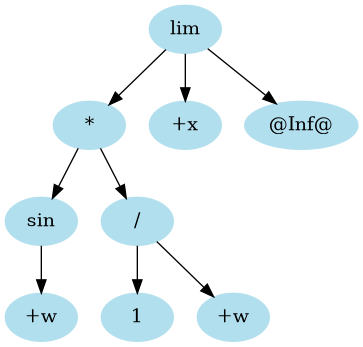
\includegraphics[width=0.8\textwidth]{pres_img/rewritten.png}
					\caption{\(\lim_{x \to +\infty}{\sin{w} \cdot \frac{1}{w}}\)}
				\end{figure}
			\end{column}
		\end{columns}
	\end{frame}

	\subsection{Terza semplificazione}
	
	\begin{frame}
		\begin{columns}
			\begin{column}{0.45\textwidth}
				\begin{figure}
					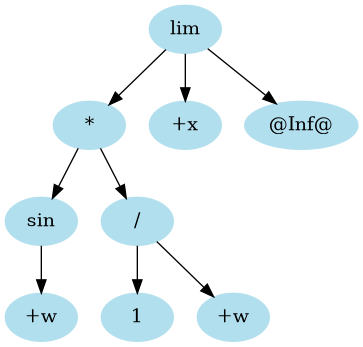
\includegraphics[width=0.8\textwidth]{pres_img/rewritten.png}
					\caption{\(\lim_{x \to +\infty}{\sin{w} \cdot \frac{1}{w}}\)}
				\end{figure}
			\end{column}
			\begin{column}{0.1\textwidth}
				\begin{center}
					$\rightarrow$
				\end{center}
			\end{column}
			\onslide<2>\begin{column}{0.45\textwidth}
				\begin{figure}
					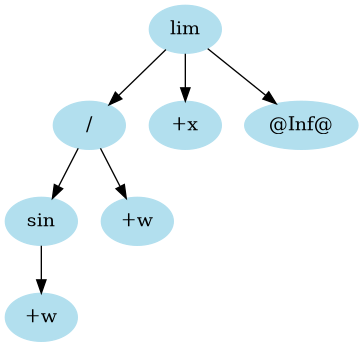
\includegraphics[width=0.8\textwidth]{pres_img/replaced2.png}
					\caption{\(\lim_{x \to +\infty}{\frac{\sin{w}}{w}}\)}
				\end{figure}
			\end{column}
		\end{columns}
	\end{frame}

	\subsection{Espressione come serie di potenze}
	
	\begin{frame}
		\frametitle{Serie di Maclaurin}
		\begin{block}{Serie di Maclaurin}
			\[
			f(x) = \sum_{n=0}^{\infty}{\frac{f^{(n)}(0)}{n!} x^{n}}
			\] 
		\end{block}
		\onslide<2>\begin{exampleblock}{Esempio}
			\[
				e^{x} = \sum_{n=0}^{\infty} \frac{x^{n}}{n!} = 1 + x + \frac{x^2}{2} + ...
			\]
			\[
				\sin{x} = \sum_{n=0}^{\infty} \frac{(-1)^{n}}{(2n + 1)!} \cdot x^{2n+1} = x - \frac{x^3}{6} + \frac{x^5}{120} + ...
			\]
		\end{exampleblock}
	\end{frame}

	\begin{frame}
		\begin{columns}
			\begin{column}{0.45\textwidth}
				\begin{figure}
					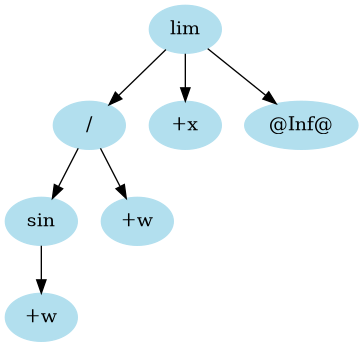
\includegraphics[width=0.8\textwidth]{pres_img/replaced2.png}
					\caption{\(\lim_{x \to +\infty}{\frac{\sin{w}}{w}}\)}
				\end{figure}
			\end{column}
			\begin{column}{0.1\textwidth}
				\begin{center}
					$\rightarrow$
				\end{center}
			\end{column}
			\onslide<2>\begin{column}{0.45\textwidth}
				\begin{figure}
					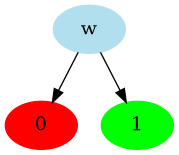
\includegraphics[width=0.4\textwidth]{pres_img/series.png}
					\caption{\(\textcolor{green}{1} \cdot w^{\textcolor{red}{0}}\)}
				\end{figure}
			\end{column}
		\end{columns}
	\end{frame}

	\subsection{Determinare il risultato}
	
	\begin{frame}
		\frametitle{Determinare il risultato}
		\begin{block}{Analisi della serie}
			Dato il primo termine della serie nella forma \(A(x)w^b\):
			\[
			\lim_{x \to x_{0}}{f(x)} = \begin{cases}
				0 &\text{if} \: b > 0 \\
				+\infty &\text{if} \: b < 0\\
				\lim_{x \to +\infty}{A(x)} &\text{if} \: b = 0
			\end{cases}
			\]
		\end{block}
	\end{frame}

	\begin{frame}
		\begin{columns}
			\begin{column}{0.45\textwidth}
				\begin{figure}
					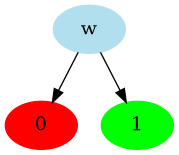
\includegraphics[width=0.4\textwidth]{pres_img/series.png}
					\caption{\(\textcolor{green}{1} \cdot w^{\textcolor{red}{0}}\)}
				\end{figure}
			\end{column}
			\begin{column}{0.1\textwidth}
				\begin{center}
					$\rightarrow$
				\end{center}
			\end{column}
			\onslide<2>\begin{column}{0.45\textwidth}
				\begin{center}
					\[
						\lim_{x \to 0}{\frac{\sin{x}}{x}} = \lim_{x \to +\infty}{1} = 1
					\]
				\end{center}
			\end{column}
		\end{columns}
	\end{frame}

	\subsection{Pattern semplificabili}
	\begin{frame}
		\frametitle{Pattern semplificabili}
		\begin{itemize}
			\pause \item \(e^{\ln{a}} \rightarrow a, \ln{e^{a}} \rightarrow a\)
			\pause \item \(\frac{a}{\frac{b}{c}} \rightarrow \frac{a \cdot c}{b}\)
			\pause \item \(a \cdot 1 \rightarrow a, \frac{a}{1} \rightarrow a, a + 0 \rightarrow a\)
			\pause \item \(\frac{1}{e^{x}} \rightarrow e^{-a}\)
			\pause \item \(\frac{1}{e^{a - b}} \rightarrow e^{b - a}\)
		\end{itemize}
	\end{frame}
	
	\subsection{L'origine del nome}
	\begin{frame}
		\frametitle{Il significato di TCAS}
		\begin{figure}
			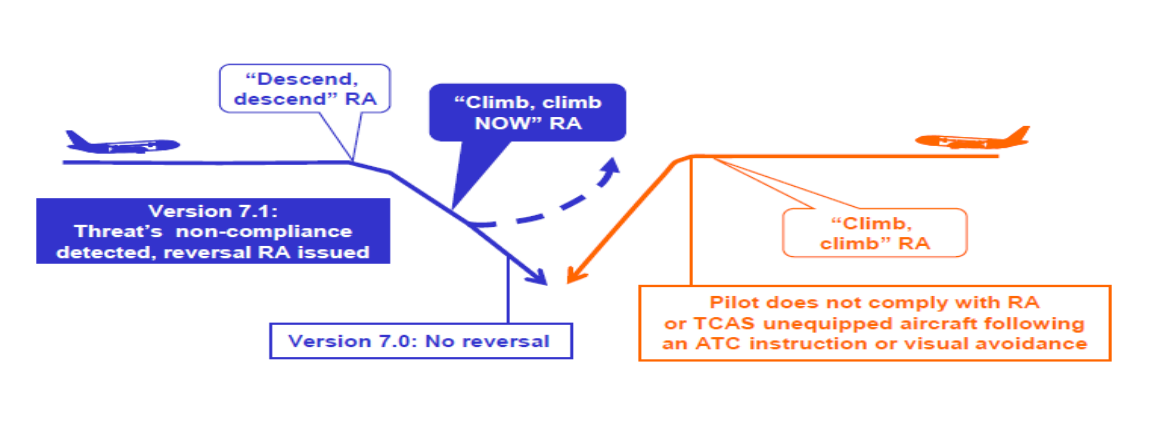
\includegraphics[width=1.0\textwidth]{pres_img/tcas.png}
		\end{figure}
	\end{frame}
	
\end{document}